
\documentclass[12pt]{article}
\usepackage{graphicx}
\usepackage{blindtext}
\usepackage{hyperref}
\usepackage[round]{natbib}   % omit 'round' option if you prefer square brackets
\bibliographystyle{apalike}

\newcommand{\midrule}{\hline}
\newcommand{\toprule}{\hline}
\newcommand{\addlinespace}{\\}
\newcommand{\bottomrule}{\hline}

\title{The depreciation of human capital evidence from Italy }
   % omit 'round' option if you prefer square brackets


\author{ Riccardo Dal Cero }

%\institute{ UCSC, Milan, Italy\\
%\email{riccardo.dalcero99@gmail.com}\\
%}

%\maketitle

%\small

%\keywords{Human Capital, Education, Gender gap, ...}

%\publishedin{Journal name, Vol. X, Issue Y, No. Z, pp. xx--yy, YEAR}
\begin{document}
\maketitle
\begin{abstract}

This study aims to estimate age-wage profiles and human capital depreciation rates for different education levels in
Italy, using a dynamic panel dataset covering the period from 1980 to 2019. Specifically, we estimate depreciation rates
for primary, secondary, and tertiary education levels, providing a comprehensive understanding of differences in human
capital depreciation. We also investigate gender differences in depreciation rates, which can have implications for
long-term economic growth and development. Our findings indicate that achieving a secondary education level compared to
lower secondary leads to a 1\% increase in the return of human capital and a 0.5\% decrease in time spent working.
Additionally, the study suggests that the gender gap in wage-age and hours-age profiles is wider for higher-educated
women, with a return on the human capital of 2.2\% per year lower, compared to men.\footnote{Total words: 4996}
\end{abstract}

\newpage
\section{Introduction}
The Ben-Porath model has been widely used in economic research to explain differences in wage-age profiles resulting
from variations in human capital. Human capital encompasses the knowledge, skills, and abilities individuals gain
through education and training, enabling them to participate in the labor market and contribute to the economy. While
human capital is subject to depreciation over time, individuals can invest in their human capital to improve it. The
difference equation that describes human capital includes a depreciation rate, a cohort-specific productivity parameter,
a curvature parameter, and age t.
\par
Numerous studies have employed the model\citet{ben1967production} to analyze cross-regional differences in wage profiles
\citet{baker1997human} and the evolution of wage inequality as in \citet{joshi2021gender} and in\citet{erosa2012human}.
However, there is still a need to explore how human capital evolves for individuals with different levels of
schooling, with a focus on potential differences in the wage profiles of women. Understanding the evolution of human
capital is crucial to identifying potential constraints to long-term economic growth as shown in \cite{mincer1981human},
as a population with higher depreciation rates and poor human capital can limit potential growth. Moreover, identifying
different returns on human capital allows us to better understand the incentive to invest in education.
\par
This paper aims to estimate the age-wage profiles and depreciation rates for different education levels while minimizing
assumptions, following Hendriks\cite{hendricks2013ben}' method $\log{y}$. Additionally, we will examine the impact of
gender discrimination on the long-term human capital of women, which can generate different returns to education. The
findings of this study will provide valuable insights into the dynamics of human capital accumulation and depreciation
in Italy. This research also informs policy interventions aimed at promoting economic growth and development by
highlighting potential constraints to long-term growth and the importance of reducing discrimination in the labor
market.
\par
Ultimately, this research contributes to the broader literature on the role of education and human capital in economic
growth and development, as well as the importance of promoting gender equality in the labor market.

\section{Empirical part}
The empirical questions that we are going to answer are the followings:
\begin{enumerate}
    \item What is the return in remuneration of human capital for different levels of education?
    \item Is there a difference in the remuneration of human capital between male and female?
\end{enumerate}
\subsection{The model predictions}
The Ben-Porath model suggests that the depreciation rate of human capital is a linear function of time and depends on
the level of human capital. This is because individuals with higher human capital face a higher depreciation rate,
similar to the relationship between capital and growth in the growth theory. As such, we can expect that individuals
with lower education levels, and therefore lower levels of human capital, will experience a lower depreciation rate
compared to those with higher levels of education. \par
In terms of the wage-age profile, individuals with lower education levels will typically invest less in human capital
and reach their maximum wage sooner and at a lower level compared to those with higher education levels. This is since individuals with higher levels of education are more likely to have skills and knowledge, which can lead
to higher wages and greater career opportunities later in their careers.
\subsection{Specification}
We use regression on the Conditional Expectation Function (CEF) as a method to estimate the relationship between the
dependent variable:
\begin{itemize}
    \item $\log{wage}_{i,t}$
    \item $\log{hours}_{i,t}$
\end{itemize}
( and  where $i$ is the individual $i$ at the age $t$) and independent variables:
\begin{itemize}
    \item $age, age^2$: the age and the age squared of the individual $i$ of the year $y$
    \item $i.cohort$ is the list of dummies of the cohorts
    \item $i.years$ is the list of dummies for the years class (class size $=5$).
\end{itemize}
while controlling for:
\begin{itemize}
    \item $educ={3,5}$ Educational level: $3:$ middle school, $5:$ High school level
    \item $female={0,1}$  Sex $(=1 if female)$
\end{itemize}

There are four specifications that we are going to use 
\begin{enumerate}
    \item   \label{spec1}    \(\log{wage}_{i,y}=   \beta_1 age_{i}+ \beta_2 age_{i}^2+i.cohort+i.years |educ={3,5}\)
    \item   \label{spec2}    \(\log{wage}_{i,y}=   \beta_1 age_{i}+ \beta_2 age_{i}^2+i.cohort+i.years |educ={3,5},sex=
    {0 (male), 1 (female)}\)
    \item  \label{spec3}    \(\log{mean(hours)}_{i,y}=  \beta_1 age_{i}+ \beta_2 age_{i}^2+i.cohort+i.years |educ={3,5}\)
    \item   \label{spec4}    \(\log{hours}_{i,y}= \beta_1 age_{i}+ \beta_2 age_{i}^2+i.cohort+i.years |educ={3,5},sex=
    {0 (male), 1 (female)}\)
\end{enumerate}
We adopt the specifications given by \citet{hendricks2013ben} denoted as \ref{spec1} and \ref{spec2}. However, we do not
include a gender fixed effect in the regression analysis, as we aim to allow gender to affect the estimates of $\eta$
and $\eta^2$ in a time-varying manner. This approach is similar to that proposed by \citet{joshi2021gender}. We also
refrain from using the month of job as a proxy for experience, as it may result in collinearity issues. The CEF method has several
limitations. 
\par
First, it assumes that the age and education variables capture all the relevant dimensions of human
capital. Other important factors, such as experience or on-the-job training, are not
explicitly considered in the model. Second, the method may suffer from omitted variable bias if there are unobserved
characteristics that affect both wages and education levels. Third, the CEF method assumes that the relationship between
age, education, and wages is linear, which may not hold in reality. 

\subsection{Identification strategy}
To estimate the depreciation rate of human capital for different levels of education, it is necessary to
implement an identification strategy that can isolate the effects of age, education, cohort, and year on wage profiles.
This section describes the identification strategy used in a study to achieve this objective.
\par
Firstly, the assumption is made that cohort effects are constant for all agents in the same 5-year cohort. This is
because individuals who are born in the same 5-year period tend to share similar social, economic, and political
experiences during their formative years. By assuming that cohort effects are constant across individuals in the same
5-year cohort, it is possible to control for unobserved heterogeneity that is specific to a particular cohort.

\par
Secondly, it is assumed that the initial human endowment is constant within the same cohort. This implies that
individuals who are born in the same 5-year cohort have similar levels of human capital at the beginning of their
careers, before investing in additional education or training. By assuming that the initial human endowment is constant
within the same cohort, it is possible to control for unobserved heterogeneity that is specific to a particular birth
cohort.

\par
Similar assumptions apply to year effects, which means that individuals within the same cohort experience the same
effects on wages over a period of 5 years. These restrictions on the model are based on some naive assumptions about the
behaviour of individuals concerning their education and human capital. For instance, it is reasonable to assume that
individuals who are born in the same 5-year cohort would have similar opportunities for education and training.
Similarly, individuals who start with the same initial human capital endowment within the same cohort are likely to face
similar labour market opportunities over time.

\par
While these assumptions may not hold perfectly in reality, they provide a useful framework for identifying the key
factors that drive the age-wage profile and depreciation rates of human capital for different levels of education in
Italy. By controlling for cohort and year effects in the analysis, it is possible to isolate the effect of age and
education on wages and estimate the rate of human capital depreciation for different groups of individuals.

\par
To estimate the depreciation rate of human capital for different levels of education, a longitudinal panel data approach
is used. Specifically, two separate OLS regressions are run for individuals with a lower-secondary education and those
with a high-school-level education, respectively. The dependent variable is the natural logarithm of the wage, and the
key independent variables are age and age squared. Cohort effects and year effects are controlled by including birth
year dummies and calendar year dummies, respectively. Additionally, the wage variable is corrected for inflation using
the consumer price index.
\par

Moreover, to examine gender differences in the evolution of human capital, four separate regressions are performed
conditioned on gender and two levels of education as in (\ref{spec2}). To capture the potential variation in gender
effects over time, the
regression on the conditional expectation function is employed. Additionally, the same method $\log{y}$ is used to
estimate the gender gap in the hours-age profile.
\par
Overall, the identification strategy used in this study allows for the separation of the effects of age, education, and
cohort on wage profiles and the estimation of the depreciation rate of human capital for different levels of education.
By using a longitudinal panel data approach and controlling for individual-specific unobserved heterogeneity and
time-varying factors, more accurate estimates of the depreciation rate of human capital can be obtained. This is a
crucial variable that affects overall economic growth and development.

\section{Data and descriptive statistics}
\subsection{Data}
The data used in this study are obtained from the Family Income Survey of the Bank of Italy, which spans a period from
1980 to 2020 with $\sim100.000 obs$. The sample comprises employees\footnote{We drop the observation for self-employed
since including would rise an issue of undereporting} both men and women born between 1940 and 2020. To expand our
sample size, we have divided the population into 15 birth cohorts, where each cohort covers five consecutive birth
years. We have also applied the same division for years, where each group includes five years. The following
table\ref{Tab:desc-cohort} tabulates the distribution of observations for the cohorts. The cohort with the highest density of
observations is cohort 10, whereas the younger and older cohorts have relatively few observations. The objective of the
study is to estimate wage-age profiles, which required the use of employee income reports merged with family and
individual statistics. To calculate $\\log{wage}_{i,t}$, we employed a series of transformations. Firstly, we summed the
monetary and non-monetary components of income. Secondly, we deflated the income figures using the Consumer Price Index
(CPI). Thirdly, we divided the income figures by the monthly hours worked and multiplied by 13 months to obtain the
annual income. Fourthly, we took the logarithm of the annual income figure. Finally, we merged the resulting dataset
with individual-level data.
\par
The process of computing $\\log{wage}_{i,t}$ was essential for the analysis, as it allowed us to measure the variation
in wages over time, which is critical for estimating wage-age profiles. By merging different datasets, we were able to
obtain a more comprehensive picture of the factors influencing wage dynamics in Italy. 
\subsection{Descriptive statistics}

The tables presented in this paper (see Tables\ref{Tab:desc-1a} and\ref{Tab:desc-1b}) provide a detailed overview of the
descriptive statistics for two key variables: the logarithm of wages and annual working hours. The tables show the mean,
standard error, and t-test for the difference in mean for each variable across four different groups based on education
level and gender. Specifically, the groups are defined by individuals with a low level of secondary school education,
and those with a secondary school education level and these subgroups are further differentiated by sex.
\par
The statistical results from the tables\ref{Tab:desc-1a}indicate that individuals with a secondary school education level tend to earn
higher wages than those with a lower level of education. Moreover, the wage gap between genders is more pronounced among
those with a secondary school education level. In other words, women tend to earn less than men across all education
levels, and the difference is wider for those with a higher level of education.
\par
Individuals with lower education tend to work more hours annually than those with higher education, while women tend to
work fewer hours than men across all education levels. However, the gender gap in working hours narrows as the level of
education increases, according to \citet{goldin}. It is worth noting that the data analyzed covers the period from 1980
to 2020, during which women's participation in the labour market increased significantly. Therefore, the actual
difference in working hours between genders may be even greater for individuals with the same characteristics.
\par
The descriptive statistics in this study of a specific cohort in 2008 show that higher education is positively
correlated with wages and a decreasing trend in working hours, potentially due to possessing skills or abilities that
increase productivity. This cohort represents middle-aged workers who have already invested significant time and
resources into their careers, so these summary statistics must be interpreted with that in mind. The findings reveal
significant disparities in labour market outcomes between individuals with different education levels and genders, with
higher-educated individuals earning more and working fewer hours. The gender gap in working hours narrows with
increasing education. (References: Table\ref{tab:desc-cohort10}, Table\ref{Tab:desc-1a}, Table\ref{Tab:desc-1b})
\section{Empirical results}
In the empirical results section, we analyze the relationship between human capital evolution and education and gender
characteristics in the labor market. Our analysis aims to answer key questions, such as the impact of secondary
education on wage age profiles and potential gender differences. We also explore how investing in human capital affects
hour-age profiles and identify potential disparities and trends in the gender gap.
\subsection{The estimation of wage age profile}
According to the human capital theory, the wage-age profile reflects the relationship between an individual's age and
their wages, which is influenced by their investment in human capital over time. To explore this relationship, we use
regression analysis with specification\ref{spec1} and present the results in Table\ref{Tab:reg1}. The key parameters
include $\beta_{age2}$, which indicates the decline in wages over time and reflects depreciation, and $\beta_{age}$,
which represents the return on investment in human capital over time. All the coefficients are statistically
significant, providing valuable insights into the dynamics of the labour market and the role of human capital investments
in shaping the wage-age profile.
\par
If we focus on individuals with lower education\ref{reg1_w_leduc}, the results indicate that an increase of one year in
age leads to an increase of $\approx 11\%$ in wages. On the other hand, for individuals with higher education
\ref{reg1_w_heduc}, an increase of one year in age leads to an increase of approximately $\approx 12.6\%$ in wages.
These findings are consistent with the human capital theory, which suggests that having a secondary level education
instead of a lower secondary education leads to higher returns, while the depreciation rate remains the same for both
groups. However, the low value of $R_{overall}^2 \approx 11\%$ suggests that the regression has very limited predictive
power, possibly due to the restrictions imposed to isolate the cohort and year-fixed effects.
\par
To visually inspect the results we show the predicted wages by cohorts.
\par
In this section, we present a graph (see Figure\ref{fig:pred_reg}) that visually depicts the relationship between
education levels and wages across different age cohorts. The results are intriguing, as they suggest that there is a
notable difference in the wage gap between older and younger cohorts. The graph shows that the wage gap is larger for
the older cohort, while the younger cohorts have a narrower difference. This finding is consistent with the notion that
higher educated individuals tend to spend part of their time endowment continuing to invest in their human capital
during the early stages of their careers, while the lower educated tend to have more experience as they started working
early, thus accumulating specialized skills. It is worth noting that this observation may indicate that specialized
skills have a higher depreciation rate and a lower return in the long term. It would be interesting to extend the model
to include two types of human capital assets: one with a higher short-term return and higher depreciation, and another
that is more costly but has lower depreciation and then let the agent choose the optimal level of the two assets
following the idea of \citet{Kruger}.
\par
The findings of our study support the theory that higher levels of human capital lead to higher wages. Specifically, the
graph\ref{fig:pred_reg} demonstrates that individuals with higher levels of education consistently earn higher wages
compared to those with lower education levels across all age cohorts. This observation highlights the importance of
investing in human capital, particularly at the early stages of one's career, to enhance earning potential in the long
term.
\par
Furthermore, the graph\ref{fig:pred_reg} also shows that the wage gap between education levels widens over time. This
suggests that younger cohorts have a smaller wage gap because the lower-educated individuals are more experienced in the
labour market, while the higher-educated individuals are just starting. However, as time goes by, the market starts
to remunerate better those individuals who have invested in higher human capital.
\par
Building upon these findings, we extend our analysis to include the effects of gender on wages by conducting a
regression analysis similar to the one before but with gender as a conditioning variable. This will allow us to examine
the gender wage gap across different education levels and age cohorts, providing important insights into the dynamics of
the labour market and the role of gender in wage determination.
\par
The results presented in Table\ref{Tab:reg2} indicate that there is clear evidence of a lower return on education for
females, with $\beta_{age, female}$ (as shown in columns(2) (4)\ref{Reg:2_L_F}) being lower than
$\beta_{age,male}$ (shown in columns (1) (3)\ref{Reg:2_L_M}). This effect is more pronounced for individuals with
higher levels of education, as the marginal gap concerning age is wider, with $\Delta_{secondary} \approx 2.2\%$
per year for those with secondary education, and $\Delta_{lower\ secondary} \approx 1.4\%$ per year for those with lower
secondary education. This result is consistent with previous research \citet{erosa2012human} and implies a lower return
on investment in human capital for females. Interestingly, there is no statistically significant difference in the
depreciation of capital over time between males and females, as $\beta_{eta^2}|female, sex = \beta_{eta^2,
female}|female,sex$ and is approximately $0.83\%$.
\par
The gender wage gap can be decomposed into two factors that widen it over time: the increase in wages as a result of
acquiring working experience, represented by $\beta_{Age}$, and the decrease in wages, represented by $\beta_{Age^2}$.
\par
These findings emphasize the importance of considering gender as a conditioning variable in wage regression analysis, as
it provides valuable insights into the dynamics of the labour market and the role of human capital investments in shaping
the wage-age profile. Moreover, the results suggest that women have lower remuneration for their human capital, which
partially explains the wide difference in wages shown in Table\ref{Tab:desc-1a}. To better understand the difference in
the evolution of wage-age profiles for women and men, we plot a chart of the predicted $\log(wage)$ comparing
individuals with the same level of education but with different genders.
\par
The chart\ref{fig:w_gend_l} illustrates that male wage-age profiles are conditional on a different level of education across
all cohorts, while the chart\ref{fig:w_gend_l_cohort8} is only for cohort 6. Now we take a look at the same results for
secondary school and lower secondary. 
\par
The chart\ref{fig:w_gend_l_cohort8} shows a higher gender gap for low educated that does not fade out as time
passes. It is important to remember that the prediction on wage is based only on the observables, thus women that drop
out of their job and stay home are not taken into account, thus the gap that we observe is only for the women that stays in
the market. Moreover, the wage gap is less accentuated for women with higher education, but this can be justified by the
fact that female that chooses to remain in the market are the ones without childbearing obligations or the ones that are
paid more.\footnote{Studying the decision to drop out of women can be useful to understand the reservation wage and thus
instrument the observability of wage; moreover the drop rates is so high that estimating the effect of having a child
for female increases the wage by 8\% this is clearly due to the fact the participation rates after first child
shrink dramatically leaving only female with higher wages and the once without child } Futhermore, the mean age in
cohort 6 is 48, thus the graph\ref{fig:w_gend_l_cohort8} approximates the gender gaps only in the neighborhood of this
age. Regardless of the strong bias due to endogeneity about the extensive margin decision, the wage age profiles for
females remains lower than man, meaning female has a lower return on the year of education compared to man.
\par
Overall the estimated return on education are consistent with the human capital theory even here the comparison was by
an individual with lower secondary and secondary education level, it would have been better the comparison with individuals
with a bachelor. However, it is not possible since they are only a few observations $\approx 600$ to get a significant
estimate of the key dependent variables. Regarding the gender differences, it is clear that there is a lower return on
human capital for females compare to men, notwithstanding this gap is strongly underestimated for the motivations written
above.

\subsection{The estimation of hour age profile}
Working hours are a fundamental variable in the human capital model, as it is the outcome of an optimization process
whereby individuals choose how much of their time endowment to allocate towards increasing their human capital, and how
much to devote to working. In this sense, working hours can be seen as a proxy for investment in human capital, as
individuals who invest more time in developing their skills and knowledge may have fewer hours available for paid
work.\par
First, we will look at the difference in the hours-age profiles for individuals with different levels of education.
Second, we will look at the difference in the hours-age profile as before but conditioning on gender. In the following
Table \ref{Tab:reg3}, we estimate with OLS the second specification \ref{spec2} for lower secondary and secondary
education levels. In column (1) \ref{Reg:3_h}, the results of the regression for the group that has achieved a secondary
school education level are reported, while in column (2) \ref{Reg:3_l}, the results of the regression on the individuals
that achieved only lower secondary school are reported.
\par
Our analysis shows that individuals with lower levels of education tend to start working earlier in life compared to
those with higher education. Indeed, the $\beta_{age}$ is positive for those who spend more time in school, while
negative\footnote{both statistically significant at 1\%}, meaning that for the higher educated, the time endowment spent in working is increasing over time with
a rate of $0.3\%$ per year.  The observation that the time spent working decreases over time with a rate of $-0.07\%$ per
year for lower-educated individuals is in line with the idea that higher-educated individuals tend to increase their
working hours over time as they invest in their human capital early in their careers, and gradually reduce their working
hours as they gain experience. This pattern is consistent with the human capital model, which predicts that individuals
with lower levels of education tend to start working earlier in life to maximize their immediate earnings, while those
with higher education may delay their entry into the labour market as they invest in their human capital.
\par
To visually inspect these results, we plot the predicted values for working hours by education level, separating each
cohort (figure.\ref{fig:hours}). This allows us to see the trends in working hours across different levels of education
for each cohort, providing further insight into the relationship between human capital and working hours
\par
In the presented graph\ref{fig:hours}, the red line represents the hours-age profiles for individuals with lower secondary school
education. These individuals tend to start spending their time endowment working earlier compared to those with
secondary education. Additionally, individuals with lower education have a higher hours-age profile, which decreases
over time. The peak of the red group's hours-age profile is reached in the early years of their working career, and then
the curve slightly decreases over time. In contrast, for those with higher education, the peak is reached between 40 and
50 years old, and then starts to decrease. It is important to emphasize that individuals with higher education spend
less time working for all years, and this trend is observed in all cohorts.
\par
To examine gender differences in the hours-age profile, we estimated the same regression model as before (specification
4), but stratified by gender. Table\ref{Reg:4_h_f} displays the results, which indicate that the slope of the hours-age
the profile is negative for individuals with higher education levels, as in the results without conditioning on gender.
However, the negative slope is flatter for women across all education levels, with a difference of only
$\Delta_{female-male}\beta_{age} \approx 0.1\%$ per year, suggesting that women tend to increase their working hours more
slowly than men. Nevertheless, low-educated women have steeper negative hours-age profiles ($\beta_{eta}|female \approx
-1.7\%$ per year) and a wider gender gap ($\Delta_{female-male}\beta_{age} \approx 1.2\%$ per year) compared to highly
educated women, implying that low-educated women tend to decrease their labour market participation faster than their
highly educated counterparts.

\par
We visually compared the predicted working hours by cohort for males and females with different levels of education.
Figure\ref{fig:h_l_cohorts} displays the predicted values of the regression of specification 4, where males with higher
education are in orange, males with lower education are in red, females with lower education are in blue, and females
with higher education are in green. We also plotted the predicted value for the middle-age cohort 7 in Figure\ref{fig:h_l_coh8}.

\par
The figure illustrates that men have higher hours-age profiles than women across all cohorts, indicating that women have
lower participation in the intensive margin compared to men, regardless of educational attainment. Additionally, for
women with lower education, the hours-age profile declines rapidly in the initial stages of their working lives,
particularly between ages 20 and 30. Consequently, the gap between low-educated females and males widens considerably
during this period, reaching its peak at around age 40. Conversely, for women who stay in school longer, there is an
increase in participation during the early stages of their careers, between ages 20 and 30, when the hours-age profile
reaches its maximum. Subsequently, the participation rate either declines or remains stable. However, it is worth noting
that the decrease in hourly worked for women is significantly underestimated since the probability of dropping out of
the labour force after having the first child is around 30% for individuals with lower and secondary school education, as
demonstrated in \citet{Bratti2005}, which implies that a large proportion of female labour force participation is
unobservable.

\par
Moreover, the gender gap in the hourly-age profile reaches its peak at around age 50 for those with higher education,
which is consistent with the idea that women who stay in school longer tend to have their first child later, delaying
their childbearing years until later in their working lives. The gap begins to decrease slightly after age 50 but
remains significant until the end of their working careers. Interestingly, the gender gap in the hourly-age profile is
wider for those who spent more time in schooling, as observed in the younger cohort. One possible explanation is that
women who pursue higher levels of education may face additional pressure to conform to traditional gender roles, such as
being a caregiver for children and elderly family members, which can lead to a reduction in their labour force
participation or hours worked. This can be particularly true during the early stages of their careers when they are
starting families or establishing themselves in their chosen fields. On the other hand, men who pursue higher education
may face fewer societal expectations to prioritize caregiving responsibilities over their careers. Thus, they may be
able to invest more time and effort into their careers.


The hours-age profiles for lower-educated women were consistently lower than for men across all cohorts, indicating that
this gender gap persists over time. However, for higher educated individuals, the gender differences were not apparent
(as shown in Figure\ref{fig:h_l_cohorts}).

Overall, our empirical findings are in line with the human capital theory, as we found a positive and statistically
significant effect of education on human capital remuneration and a concave wage-age profile as predicted by the model
with depreciation $\Delta > 0$. Additionally, the hours-age profile supports the human capital model's predictions, with
higher-educated individuals having an increasing hours-age profile, and lower-educated individuals having a decreasing
one. Furthermore, our analysis of the gender gap in the hours-age profile shows that women tend to have lower
participation in the intensive margin compared to men, regardless of their level of educational attainment. The gap is
wider for lower-educated women, and it decreases slightly for higher-educated women after the age of 50, which is
consistent with the fact that they tend to have their first child later and shift childbearing years later in their
working life. It is also interesting to note that the gender gap in the hourly-age profile at the beginning of the
career is wider for those who spent more time in schooling, as seen in the younger cohort. These findings provide
insights into the complex interplay between education, gender, and labour market outcomes.
\section{Conclusions}
In conclusion, this paper has provided an analysis of the gender wage gap in a European country, focusing on the role of
education and human capital. The empirical findings are consistent with the human capital theory, as we observe a
positive statistically significant effect of education on the remuneration of human capital and a concave shape of the
wage-age profile, in line with the model with $\Delta > 0$.
\par
Furthermore, the analysis shows that the gender wage gap widens over time, mainly due to differences in the remuneration
of human capital between men and women. Women have a lower remuneration of human capital, even for the same level of
education, which can be partly explained by differences in working hours, as women tend to invest less time in
developing their skills and knowledge.
\par
The results also indicate that individuals with lower levels of education start working earlier, to maximize their immediate earnings, while those with higher levels of education may take longer to start working as
they invest in their human capital (as in \citet{yoram}). This is reflected in the hours-age profile, which decreases over time for those with
lower education, while it increases for those with higher education.
\par
However, it is important to note that the analysis has certain limitations. Firstly, the restriction imposed on cohort
fixed effects and years fixed effects, may not capture all the heterogeneity in the data. Secondly, the analysis
only focuses on a single country, and the results may not be generalizable to other contexts. Finally, the study does
not account for the potential impact of discrimination and other factors that may contribute to the gender wage gap.
\par
Overall, this study provides insights into the factors that contribute to the gender wage gap and highlights the
importance of education and human capital in determining individuals' earnings. Further research is needed to explore
the role of other factors, such as discrimination and family responsibilities, and to investigate the effectiveness of
policies aimed at reducing the gender wage gap.






\newpage
\medskip
\bibliography{ref}
\newpage
\section{Tables and figures}
\begin{center}
    \begin{table}[htbp]\centering
    \def\sym#1{\ifmmode^{#1}\else\(^{#1}\)\fi}
    \caption{\label{Tab:desc-1a}Descriptive statistics wages}
    \begin{tabular}{l*{4}{c}}
        \hline

        \multicolumn{1}{c}{Education level}   &\multicolumn{1}{c}{Male}&\multicolumn{1}{c}{Female}&\multicolumn{1}{c}{Diff.}\\
                        \\
        \hline
        Lower Secondary &       51.71           &    48.06          &   3.642061\sym{***} \\
                        &       (33.06)         &   (40.60)         &  (.9713213)       \\
        Secondary       &       124.03          &    113.09         &   5.360341\sym{***}   \\
                        &       (91.37)         &   (73.14)         &   (.5809988 )       \\
        Diff.           &       -18.47816\sym{***} &   -16.75988\sym{***} &                      \\
                        &       (.7922257)  &   (1.07596)           &                       \\
        \\
        \hline
        \multicolumn{3}{l}{\footnotesize Standard errors in parentheses}\\
        \multicolumn{3}{l}{\footnotesize }\\
        \multicolumn{3}{l}{\footnotesize \sym{*} \(p<0.10\), \sym{**} \(p<0.05\), \sym{***} \(p<0.01\)}\\

    \end{tabular}
\end{table}
\begin{table}[htbp]\centering
    \def\sym#1{\ifmmode^{#1}\else\(^{#1}\)\fi}
    \caption{\label{Tab:desc-1b}Descriptive statistics annual working hours}
    \begin{tabular}{l*{4}{c}}
        \hline
        \multicolumn{1}{c}{Education level}   &\multicolumn{1}{c}{Male}&\multicolumn{1}{c}{Female}&\multicolumn{1}{c}{Diff}\\
        \\
        \hline
            Lower Secondary & 1,952.12      & 1,642.11& 310.0051\sym{***}  \\
                            & (393.85)      & (537.70)& (12.13044)  \\
            Secondary       &  1,811.48     & 1,507.51& 253.783\sym{***}      \\
                            & (484.11)      & (491.03)& (4.887414)    \\
            Diff.           &       27.01869 \sym{***}   & -29.20347\sym{***}\\
                            &       (6.180364)  &   (11.81991)  \\
        \\                    
        \hline
        \multicolumn{3}{l}{\footnotesize Standard errors in parentheses}\\
        \multicolumn{3}{l}{\footnotesize }\\
        \multicolumn{3}{l}{\footnotesize \sym{*} \(p<0.10\), \sym{**} \(p<0.05\), \sym{***} \(p<0.01\)}\\


    \end{tabular}
\end{table}

    \begin{tabular}{l*{6}{c}}
\toprule
                &   no edu&  primary&lower secondary&secondary technical - 3 years&secondary&first level degree\\
\midrule
Mean of log(wage)&     3.61&     3.63&     3.67&     3.69&     3.75&     3.66\\
                &      (.)&   (0.06)&   (0.03)&   (0.02)&   (0.02)&   (0.06)\\
\addlinespace
Mean of work hour& 1,920.00& 1,886.70& 1,811.86& 1,780.06& 1,678.31& 1,828.11\\
                &      (.)& (116.59)&  (50.03)&  (31.46)&  (38.77)& (116.77)\\
\addlinespace
mean\_y          & 71261.03& 71261.03& 71261.03& 71261.03& 71261.03& 71261.03\\
                &      (.)&   (0.00)&   (0.00)&   (0.00)&   (0.00)&   (0.00)\\
\addlinespace
Sex             &     0.00&     0.26&     0.40&     0.55&     0.66&     0.57\\
                &      (.)&   (0.45)&   (0.49)&   (0.50)&   (0.48)&   (0.53)\\
\bottomrule
\end{tabular}

    {
\def\sym#1{\ifmmode^{#1}\else\(^{#1}\)\fi}
\begin{tabular}{l*{5}{c}}
\hline
            &\multicolumn{1}{c}{(Cohort)} & \multicolumn{1}{c}{N.obs} & & \multicolumn{1}{c}{Freq.}& \multicolumn{1}{c}{Perc.} & \multicolumn{1}{c}{Cum.}\\
\hline
1           &          42         & 0.04      &  0.04\\
            &                     \\

2           &         619    &0.59     &   0.63       \\
            &                     \\

3           &        1816    & 1.74     &   2.37    \\
            &                     \\

4           &        3333   & 3.20   &     5.57     \\
            &                     \\

5           &        6869    &6.58     &  12.15     \\
            &                     \\

6           &        9495    &9.10   &    21.26     \\
            &                     \\

7           &       11401     &10.93   &    32.19    \\
            &                     \\

8           &       11971    &11.48      & 43.66     \\
            &                     \\

9           &       13347    &12.79     &  56.46     \\
            &                     \\

10          &       14240    & 13.65  &     70.11    \\
            &                     \\

11          &       10862  & 10.41   &    80.52      \\
            &                     \\

12          &        8222    &7.88    &   88.40     \\
            &                     \\

13          &        6291  &6.03  &     94.43       \\
            &                     \\

14          &        4291  &  4.11  &     98.55     \\
            &                     \\

15          &        1517   & 1.45 &     100.00      \\
            &                     \\
\hline
Total       &      104316         \\
            &                     \\

\multicolumn{2}{l}{\footnotesize \textit{t} statistics in parentheses}\\
\multicolumn{2}{l}{\footnotesize \sym{*} \(p<0.05\), \sym{**} \(p<0.01\), \sym{***} \(p<0.001\)}\\
\end{tabular}
}

    \begin{table}[htbp]\centering
\def\sym#1{\ifmmode^{#1}\else\(^{#1}\)\fi}
\caption{Regression table \label{reg1}}
\begin{tabular}{l*{2}{c}}
\toprule
                    &\multicolumn{1}{c}{(1)}         &\multicolumn{1}{c}{(2)}         \\
\midrule
Age                 &       0.126\sym{***}&       0.109\sym{***}\\
                    &     (0.018)         &     (0.006)         \\
                    \\
                    Cohort f.e           &       Yes        &      Yes \\
                                                \\
                    \addlinespace
                    years f.e.            &       Yes         &       Yes         \\
                                               \\
                    \addlinespace
Constant            &      -0.199         &       0.038         \\
                    &     (0.784)         &     (0.475)         \\
\midrule
Observations        &       10088         &       28968         \\
\bottomrule
\multicolumn{3}{l}{\footnotesize Standard errors in parentheses}\\
\multicolumn{3}{l}{\footnotesize }\\
\multicolumn{3}{l}{\footnotesize \sym{*} \(p<0.10\), \sym{**} \(p<0.05\), \sym{***} \(p<0.01\)}\\
\end{tabular}
\end{table}

    \begin{table}[htbp]\centering
    \def\sym#1{\ifmmode^{#1}\else\(^{#1}\)\fi}
    \caption{Regression table \label{reg2}}
    \begin{tabular}{l*{4}{c}}
    \hline
                        &\multicolumn{1}{c}{(1) M. L.Sec.}\label{2.a_m_ls}         &\multicolumn{1}{c}{(2) M.
                        Sec.}\label{2.a_m_s}        &\multicolumn{1}{c}{(3)F. L.Sec.}\label{2.a_f_ls}        &\multicolumn{1}{c}{(4)F.
                        Sec}\label{2.a_f_s}
                        \\
    \hline
    Age                 &     0.13526\sym{***}&     0.11087\sym{***}&     0.10669\sym{***}&     0.09855\sym{***}\\
                        &   (0.03060)         &   (0.01950)         &   (0.00757)         &   (0.00999)         \\
    \\
    age2                &    -0.00087\sym{***}&    -0.00081\sym{***}&    -0.00087\sym{***}&    -0.00068\sym{***}\\
                        &   (0.00032)         &   (0.00021)         &   (0.00008)         &   (0.00010)         \\
    \\
    Cohort fixed effect           &       Yes        &       Yes      & Yes & Yes  \\
    Years (5 year class) fixed effect             &       Yes       &       Yes      & Yes  & Yes   \\
    \hline
    Observations        &        4669         &        5626         &       19337         &       10114         \\
    \hline
    \multicolumn{5}{l}{\footnotesize Standard errors in parentheses}\\
    \multicolumn{5}{l}{\footnotesize }\\
    \multicolumn{5}{l}{\footnotesize \sym{*} \(p<0.10\), \sym{**} \(p<0.05\), \sym{***} \(p<0.01\)}\\
    \end{tabular}
    \end{table}
    
    \begin{table}[htbp]\centering
\def\sym#1{\ifmmode^{#1}\else\(^{#1}\)\fi}
\caption{Regression \(E[log(Hours)|educ]\) \label{Tab:reg3}}
\begin{tabular}{l*{2}{c}}
\toprule
                    &\multicolumn{1}{c}{(1)\(educ=1\)\label{Reg:3_h}}         &\multicolumn{1}{c}{\(educ=0\)\label{Reg:3_l}}         \\
\midrule
Age                 &       0.031\sym{***}&      -0.007\sym{***}\\
                    &     (0.003)         &     (0.000)         \\
\addlinespace
age2                &      -0.000\sym{***}&       0.000\sym{***}\\
                    &     (0.000)         &     (0.000)         \\
\addlinespace
age2                &      -0.000\sym{*}  &       0.000         \\
                    &     (0.000)         &     (0.000)         \\
\\
Cohort f.e           &       Yes        &      Yes \\
                            \\
\addlinespace
years f.e.            &       Yes         &       Yes         \\
                           \\
\addlinespace
Constant            &       6.786\sym{***}&       7.833\sym{***}\\
                    &     (0.166)         &     (0.020)         \\
\midrule
Observations        &       10088         &       28968         \\
$R^2$ overall       &   0.0345&0.3897 \\
\bottomrule
\multicolumn{3}{l}{\footnotesize Standard errors in parentheses}\\
\multicolumn{3}{l}{\footnotesize }\\
\multicolumn{3}{l}{\footnotesize \sym{*} \(p<0.10\), \sym{**} \(p<0.05\), \sym{***} \(p<0.01\)}\\
\end{tabular}
\end{table}

    \begin{table}[htbp]\centering
\def\sym#1{\ifmmode^{#1}\else\(^{#1}\)\fi}
\caption{Regression table \label{reg4}}
\begin{tabular}{l*{4}{c}}
\toprule
                    &\multicolumn{1}{c}{(1)}         &\multicolumn{1}{c}{(2)}         &\multicolumn{1}{c}{(3)}         &\multicolumn{1}{c}{(4)}         \\
\midrule
Age                 &     0.00664\sym{***}&     0.00428\sym{***}&    -0.00655\sym{***}&    -0.00689\sym{***}\\
                    &   (0.00084)         &   (0.00073)         &   (0.00024)         &   (0.00034)         \\
\addlinespace
age2                &    -0.00006\sym{***}&    -0.00003\sym{***}&     0.00003\sym{***}&     0.00004\sym{***}\\
                    &   (0.00001)         &   (0.00001)         &   (0.00000)         &   (0.00000)         \\
\addlinespace
Cohort=1            &     0.00000         &     0.00000         &     0.00000         &     0.00000         \\
                    &         (.)         &         (.)         &         (.)         &         (.)         \\
\addlinespace
Cohort=2            &    -0.10875\sym{***}&    -0.10144\sym{**} &     0.02052         &    -0.00604         \\
                    &   (0.02585)         &   (0.04229)         &   (0.01927)         &   (0.05698)         \\
\addlinespace
Cohort=3            &    -0.03457         &    -0.04720         &    -0.01953         &    -0.02148         \\
                    &   (0.02497)         &   (0.04103)         &   (0.01895)         &   (0.05504)         \\
\addlinespace
Cohort=4            &    -0.13421\sym{***}&    -0.13423\sym{***}&    -0.03231\sym{*}  &    -0.02966         \\
                    &   (0.02515)         &   (0.04082)         &   (0.01892)         &   (0.05493)         \\
\addlinespace
Cohort=5            &    -0.12895\sym{***}&    -0.10977\sym{***}&    -0.06005\sym{***}&    -0.05568         \\
                    &   (0.02558)         &   (0.04094)         &   (0.01898)         &   (0.05494)         \\
\addlinespace
Cohort=6            &    -0.10098\sym{***}&    -0.08635\sym{**} &    -0.08488\sym{***}&    -0.07619         \\
                    &   (0.02629)         &   (0.04125)         &   (0.01910)         &   (0.05501)         \\
\addlinespace
Cohort=7            &    -0.10419\sym{***}&    -0.08325\sym{**} &    -0.09141\sym{***}&    -0.07899         \\
                    &   (0.02712)         &   (0.04169)         &   (0.01927)         &   (0.05512)         \\
\addlinespace
Cohort=8            &    -0.07086\sym{**} &    -0.04956         &    -0.11222\sym{***}&    -0.09736\sym{*}  \\
                    &   (0.02813)         &   (0.04224)         &   (0.01947)         &   (0.05526)         \\
\addlinespace
Cohort=9            &    -0.05504\sym{*}  &    -0.04042         &    -0.13059\sym{***}&    -0.11586\sym{**} \\
                    &   (0.02922)         &   (0.04282)         &   (0.01969)         &   (0.05542)         \\
\addlinespace
Cohort=10           &    -0.03127         &    -0.01890         &    -0.15453\sym{***}&    -0.13872\sym{**} \\
                    &   (0.03048)         &   (0.04347)         &   (0.01995)         &   (0.05560)         \\
\addlinespace
Cohort=11           &    -0.05609\sym{*}  &    -0.02720         &    -0.16540\sym{***}&    -0.14791\sym{***}\\
                    &   (0.03172)         &   (0.04420)         &   (0.02021)         &   (0.05579)         \\
\addlinespace
Cohort=12           &    -0.04494         &    -0.01918         &    -0.20371\sym{***}&    -0.18665\sym{***}\\
                    &   (0.03305)         &   (0.04493)         &   (0.02052)         &   (0.05601)         \\
\addlinespace
Cohort=13           &    -0.05757\sym{*}  &    -0.03701         &    -0.22877\sym{***}&    -0.20986\sym{***}\\
                    &   (0.03451)         &   (0.04579)         &   (0.02087)         &   (0.05627)         \\
\addlinespace
Cohort=14           &    -0.01332         &    -0.00896         &    -0.28138\sym{***}&    -0.26166\sym{***}\\
                    &   (0.03634)         &   (0.04685)         &   (0.02121)         &   (0.05651)         \\
\addlinespace
years=1             &     0.00000         &     0.00000         &     0.00000         &     0.00000         \\
                    &         (.)         &         (.)         &         (.)         &         (.)         \\
\addlinespace
years=2             &     0.01534\sym{***}&     0.00525         &    -0.00064         &    -0.00326\sym{*}  \\
                    &   (0.00355)         &   (0.00335)         &   (0.00126)         &   (0.00180)         \\
\addlinespace
years=3             &     0.04231\sym{***}&     0.03728\sym{***}&     0.00662\sym{***}&     0.00285         \\
                    &   (0.00488)         &   (0.00444)         &   (0.00178)         &   (0.00255)         \\
\addlinespace
years=4             &     0.03696\sym{***}&     0.02753\sym{***}&     0.02034\sym{***}&     0.01552\sym{***}\\
                    &   (0.00657)         &   (0.00594)         &   (0.00243)         &   (0.00345)         \\
\addlinespace
years=5             &     0.02608\sym{***}&     0.01363\sym{*}  &     0.02264\sym{***}&     0.02156\sym{***}\\
                    &   (0.00858)         &   (0.00770)         &   (0.00322)         &   (0.00452)         \\
\addlinespace
years=6             &     0.01209         &     0.00031         &    -0.00049         &    -0.01338\sym{**} \\
                    &   (0.01015)         &   (0.00901)         &   (0.00382)         &   (0.00539)         \\
\addlinespace
Cohort=15           &                     &                     &    -0.06478\sym{***}&    -0.05879         \\
                    &                     &                     &   (0.02161)         &   (0.05680)         \\
\addlinespace
Constant            &     7.30019\sym{***}&     7.32478\sym{***}&     7.83727\sym{***}&     7.82594\sym{***}\\
                    &   (0.03770)         &   (0.04731)         &   (0.02118)         &   (0.05648)         \\
\midrule
Observations        &        5293         &        6370         &       26561         &       16663         \\
\bottomrule
\multicolumn{5}{l}{\footnotesize Standard errors in parentheses}\\
\multicolumn{5}{l}{\footnotesize }\\
\multicolumn{5}{l}{\footnotesize \sym{*} \(p<0.10\), \sym{**} \(p<0.05\), \sym{***} \(p<0.01\)}\\
\end{tabular}
\end{table}

\end{center}

\newpage

\begin{center}
    

\begin{figure}[h]
    \centering
    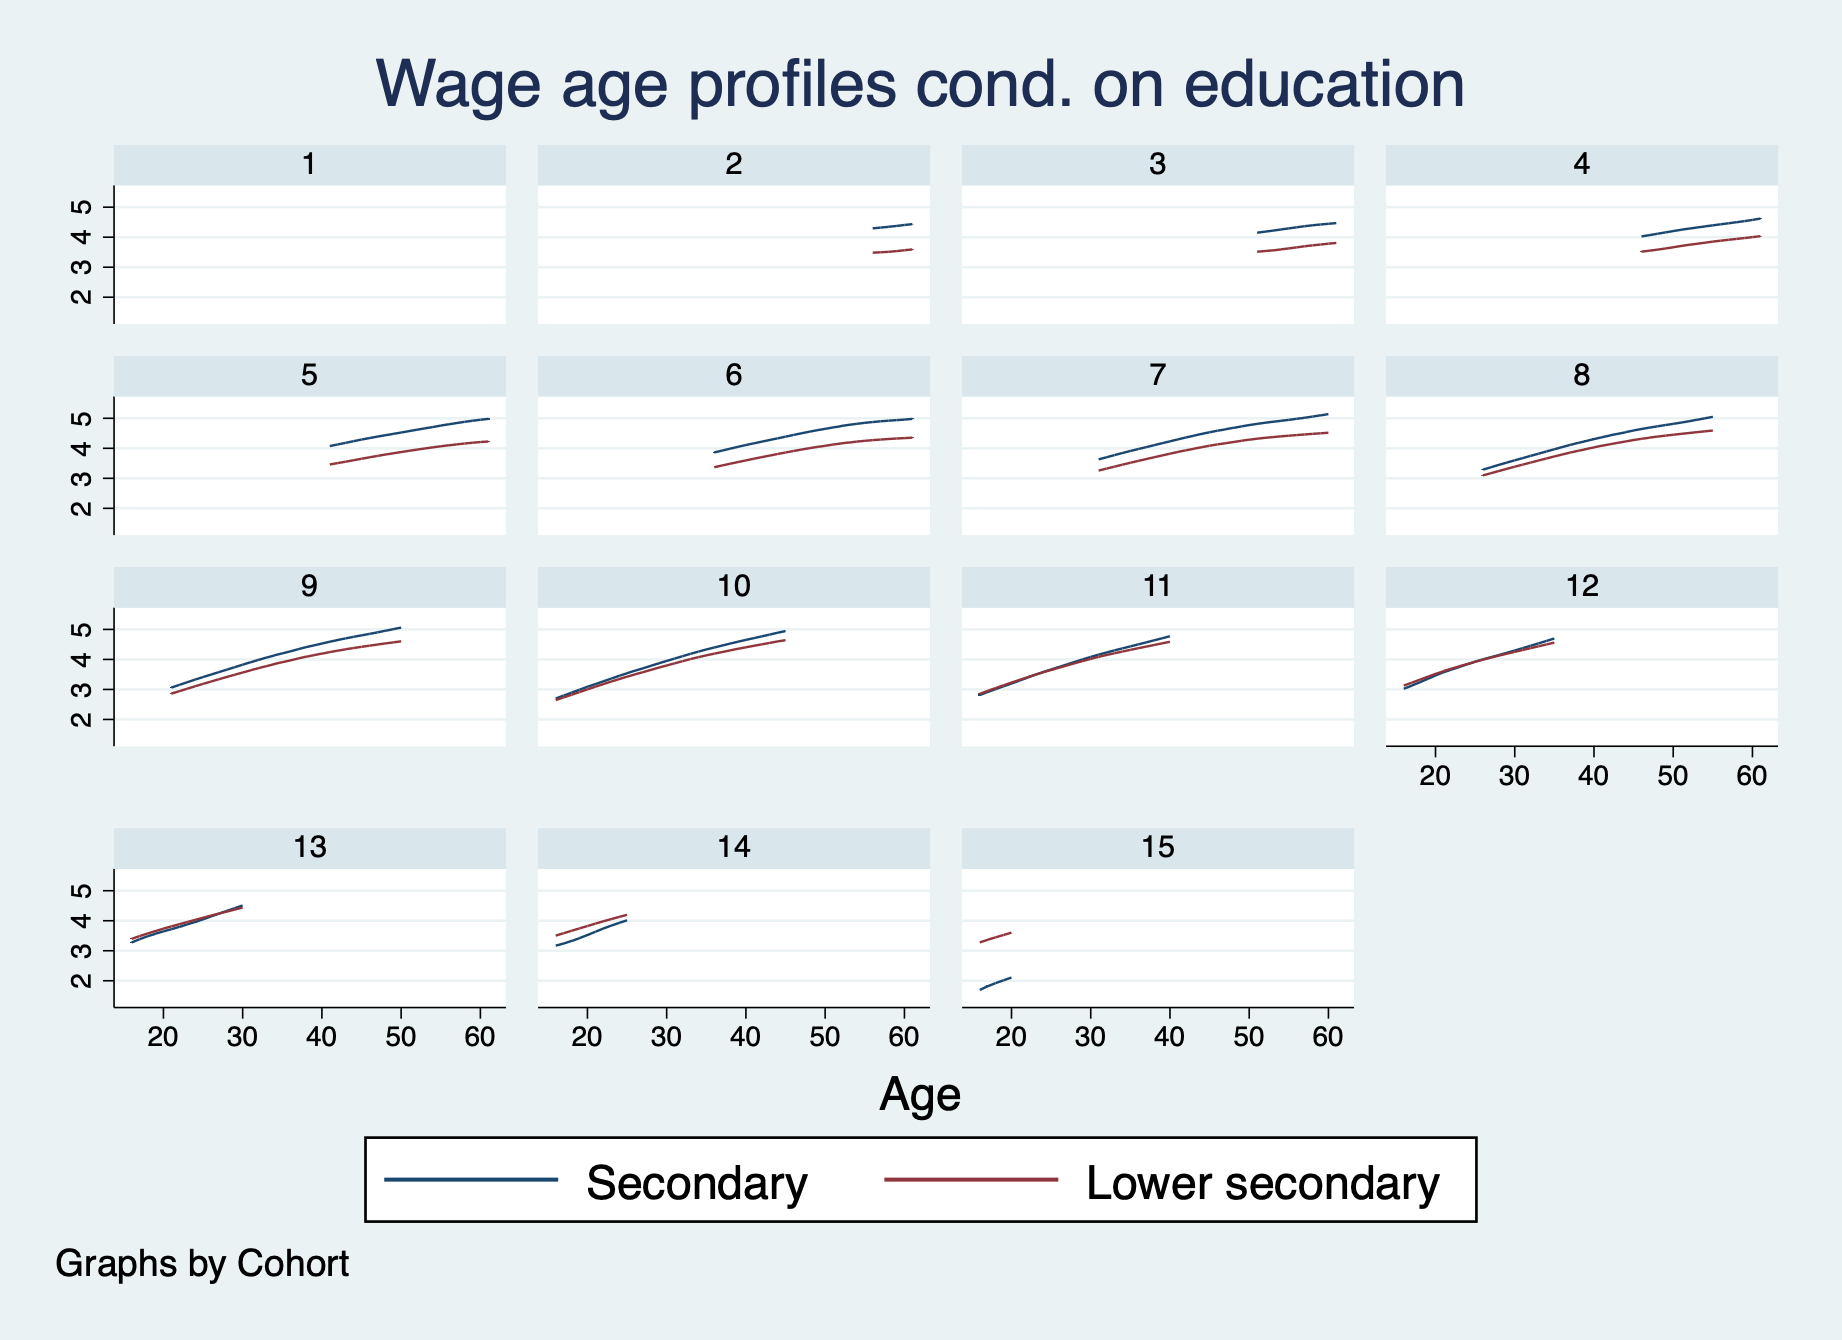
\includegraphics[scale=0.4]{graph1.png}
    \caption{\label{fig:pred_reg}Predicted wage-age profiles by cohort}
\end{figure}
\begin{figure}[!h]
    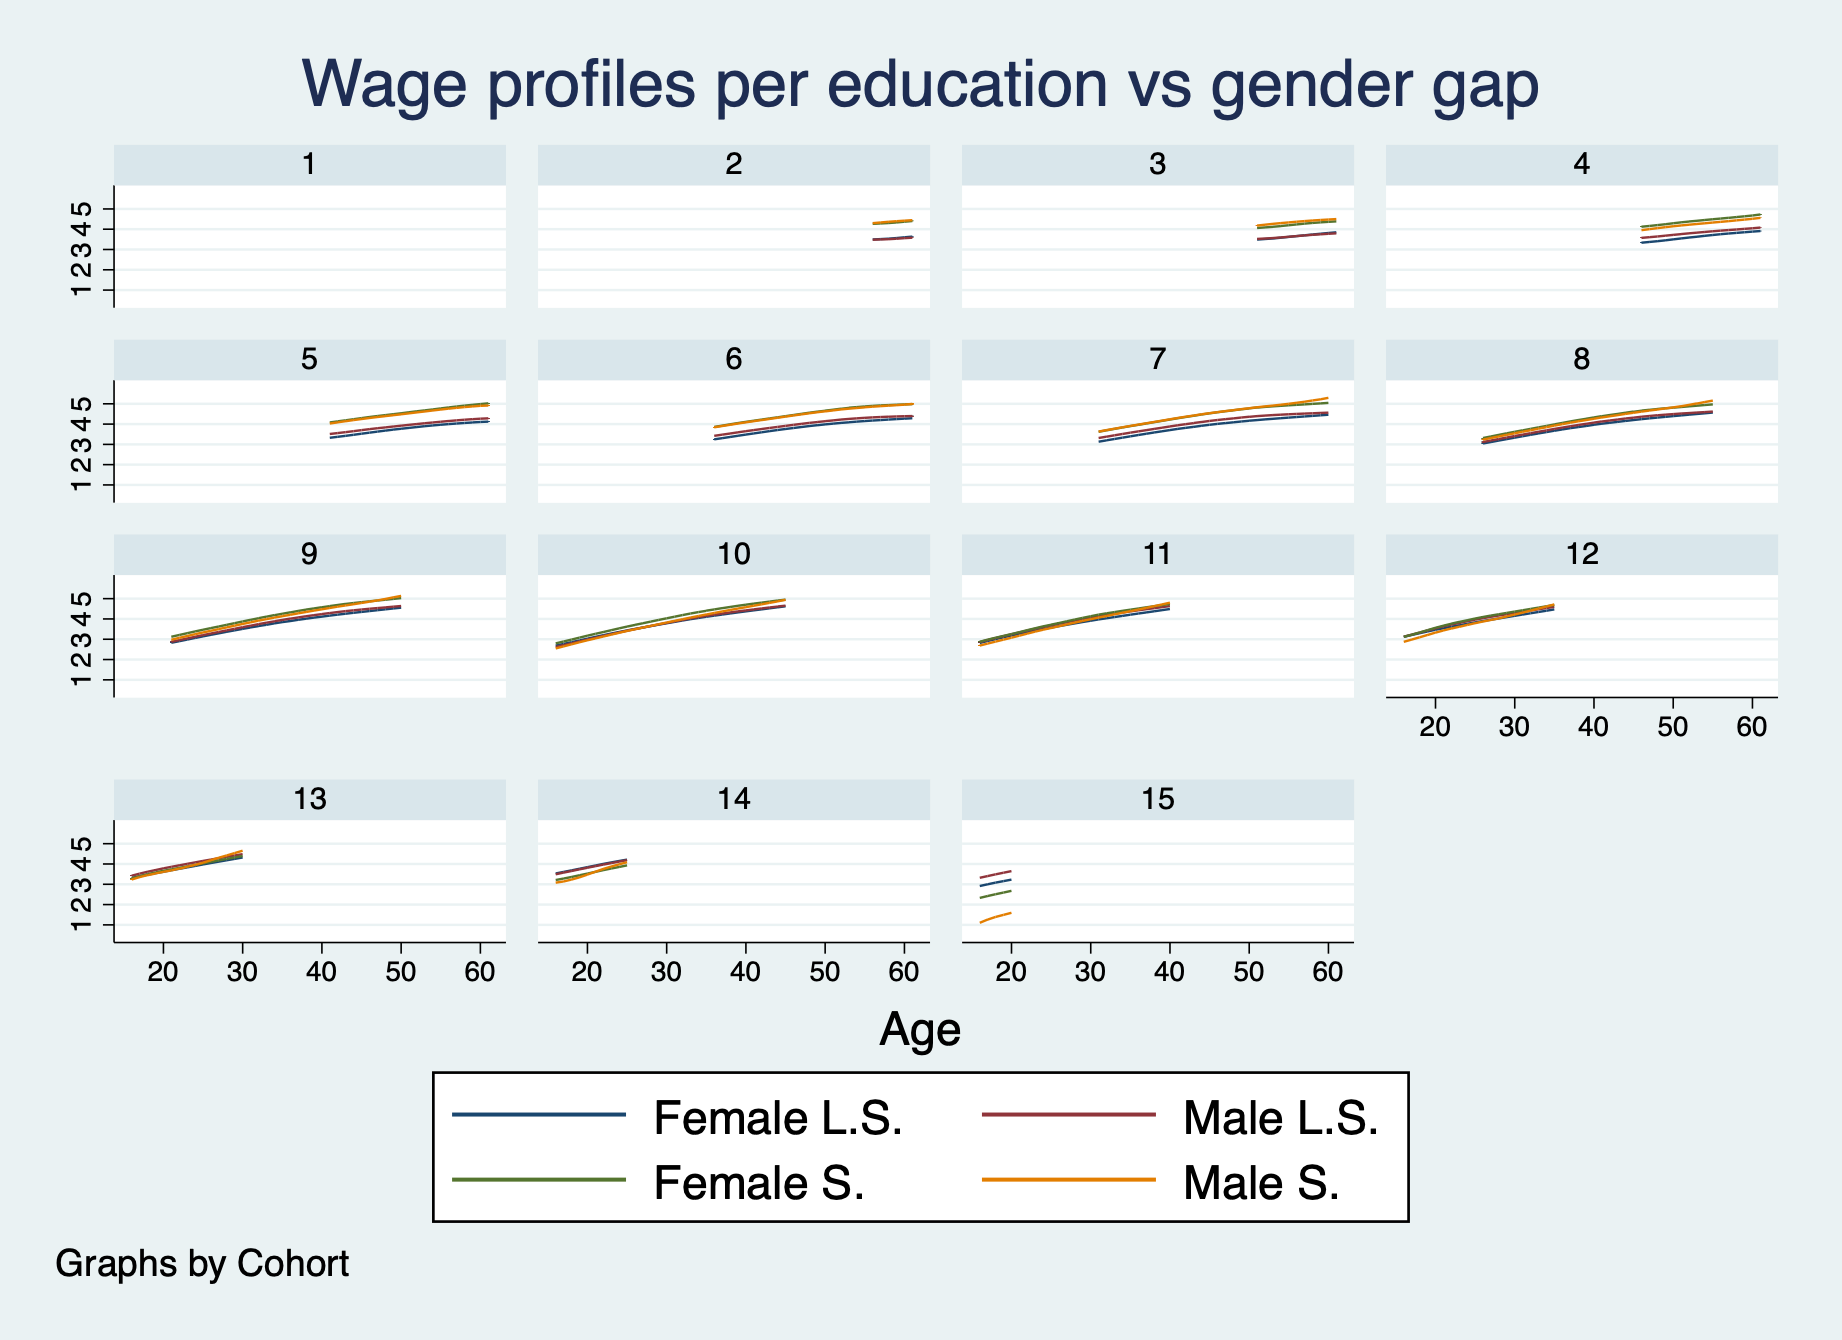
\includegraphics[scale=0.4]{graph2.png}
    \caption{\label{fig:w_gend_l}Gender gap in the wage age profiles for different education level}
\end{figure}
\begin{figure}[!h]
    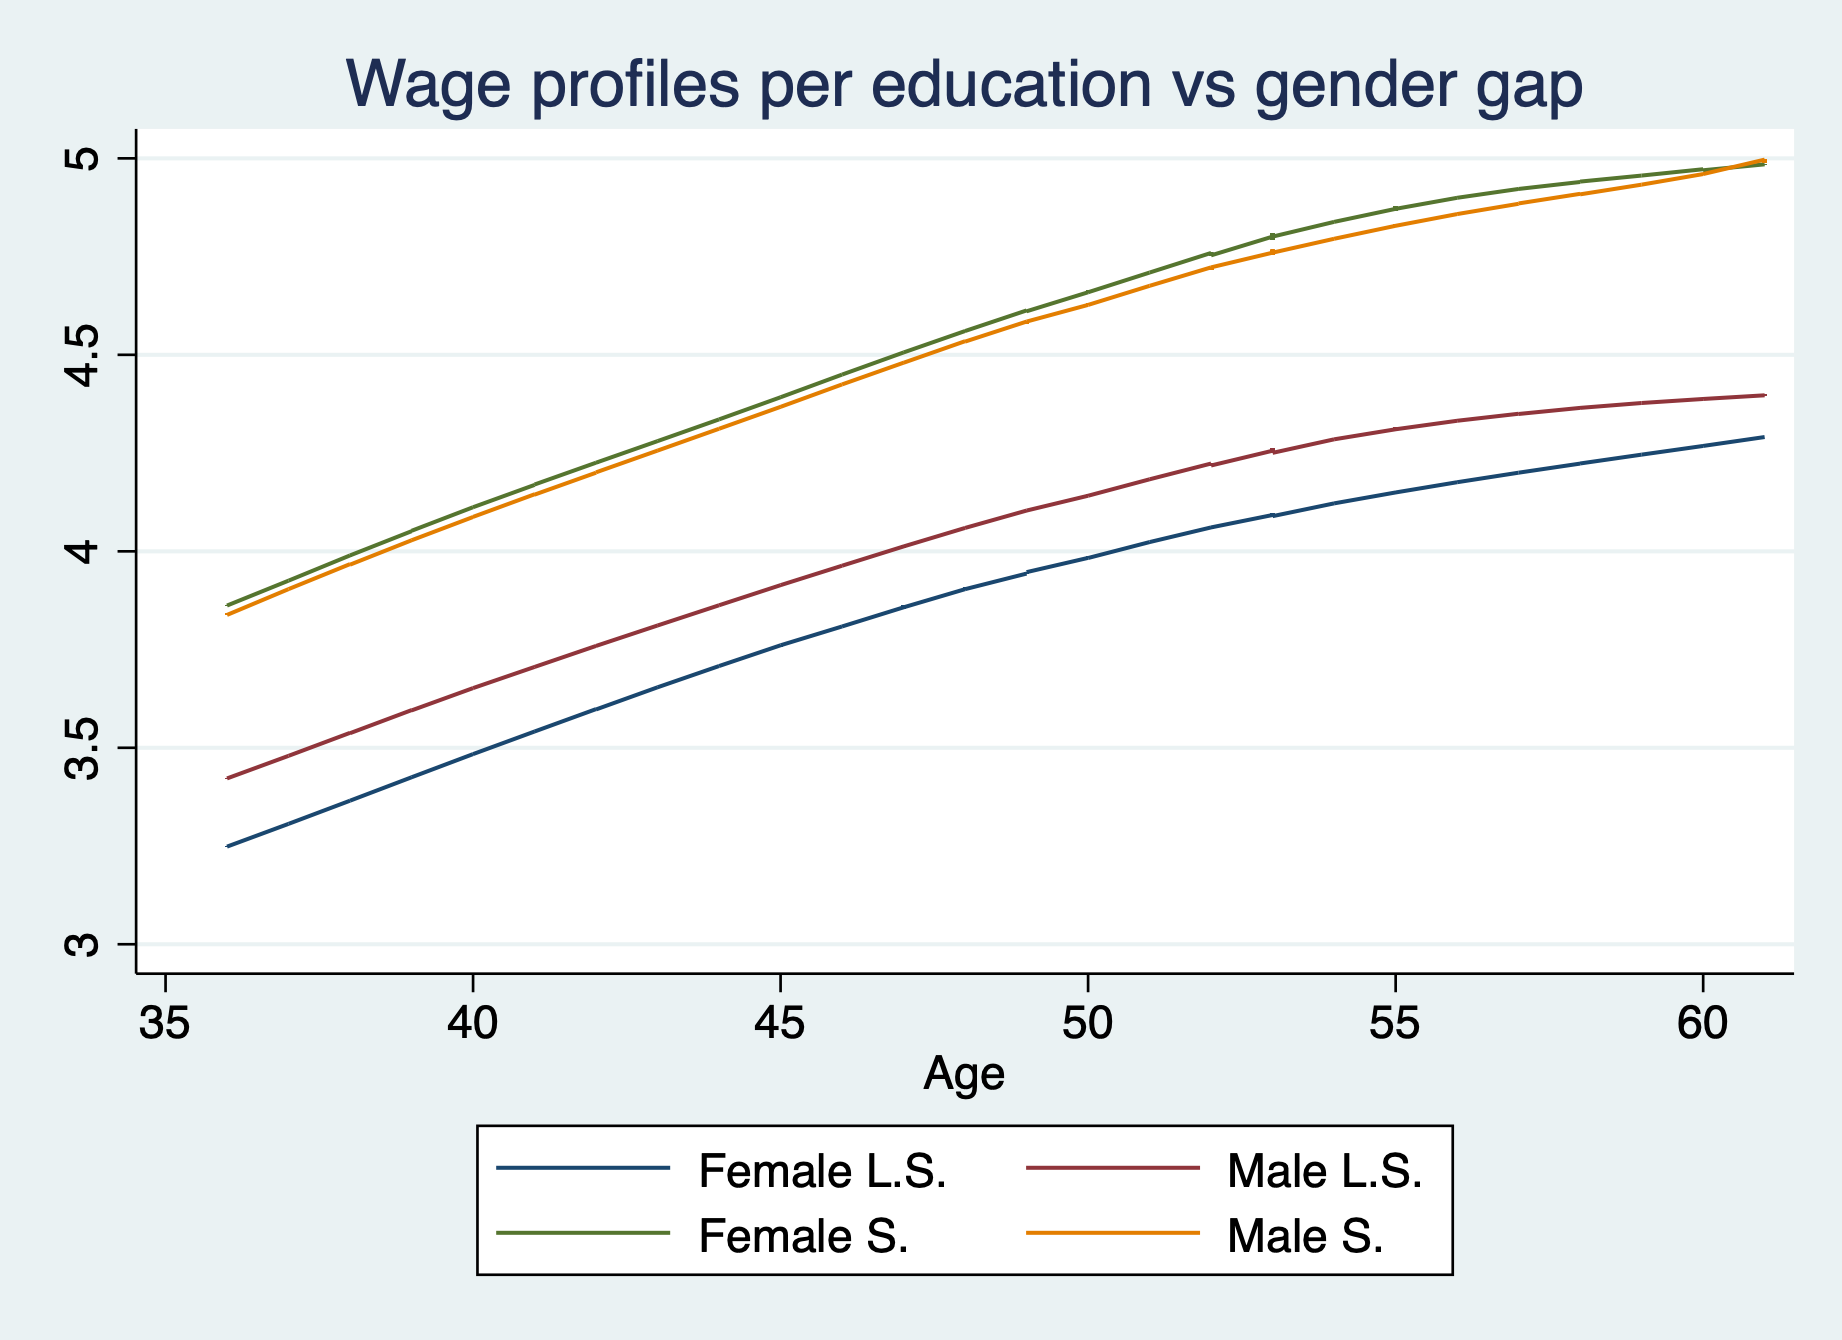
\includegraphics[scale=0.4]{graph2_1.png}
    \caption{\label{fig:w_gend_l_cohort8}Gender gap in the wage age profiles for different education level in the cohort
    8}
\end{figure}
\begin{figure}[!h]    
    \centering
    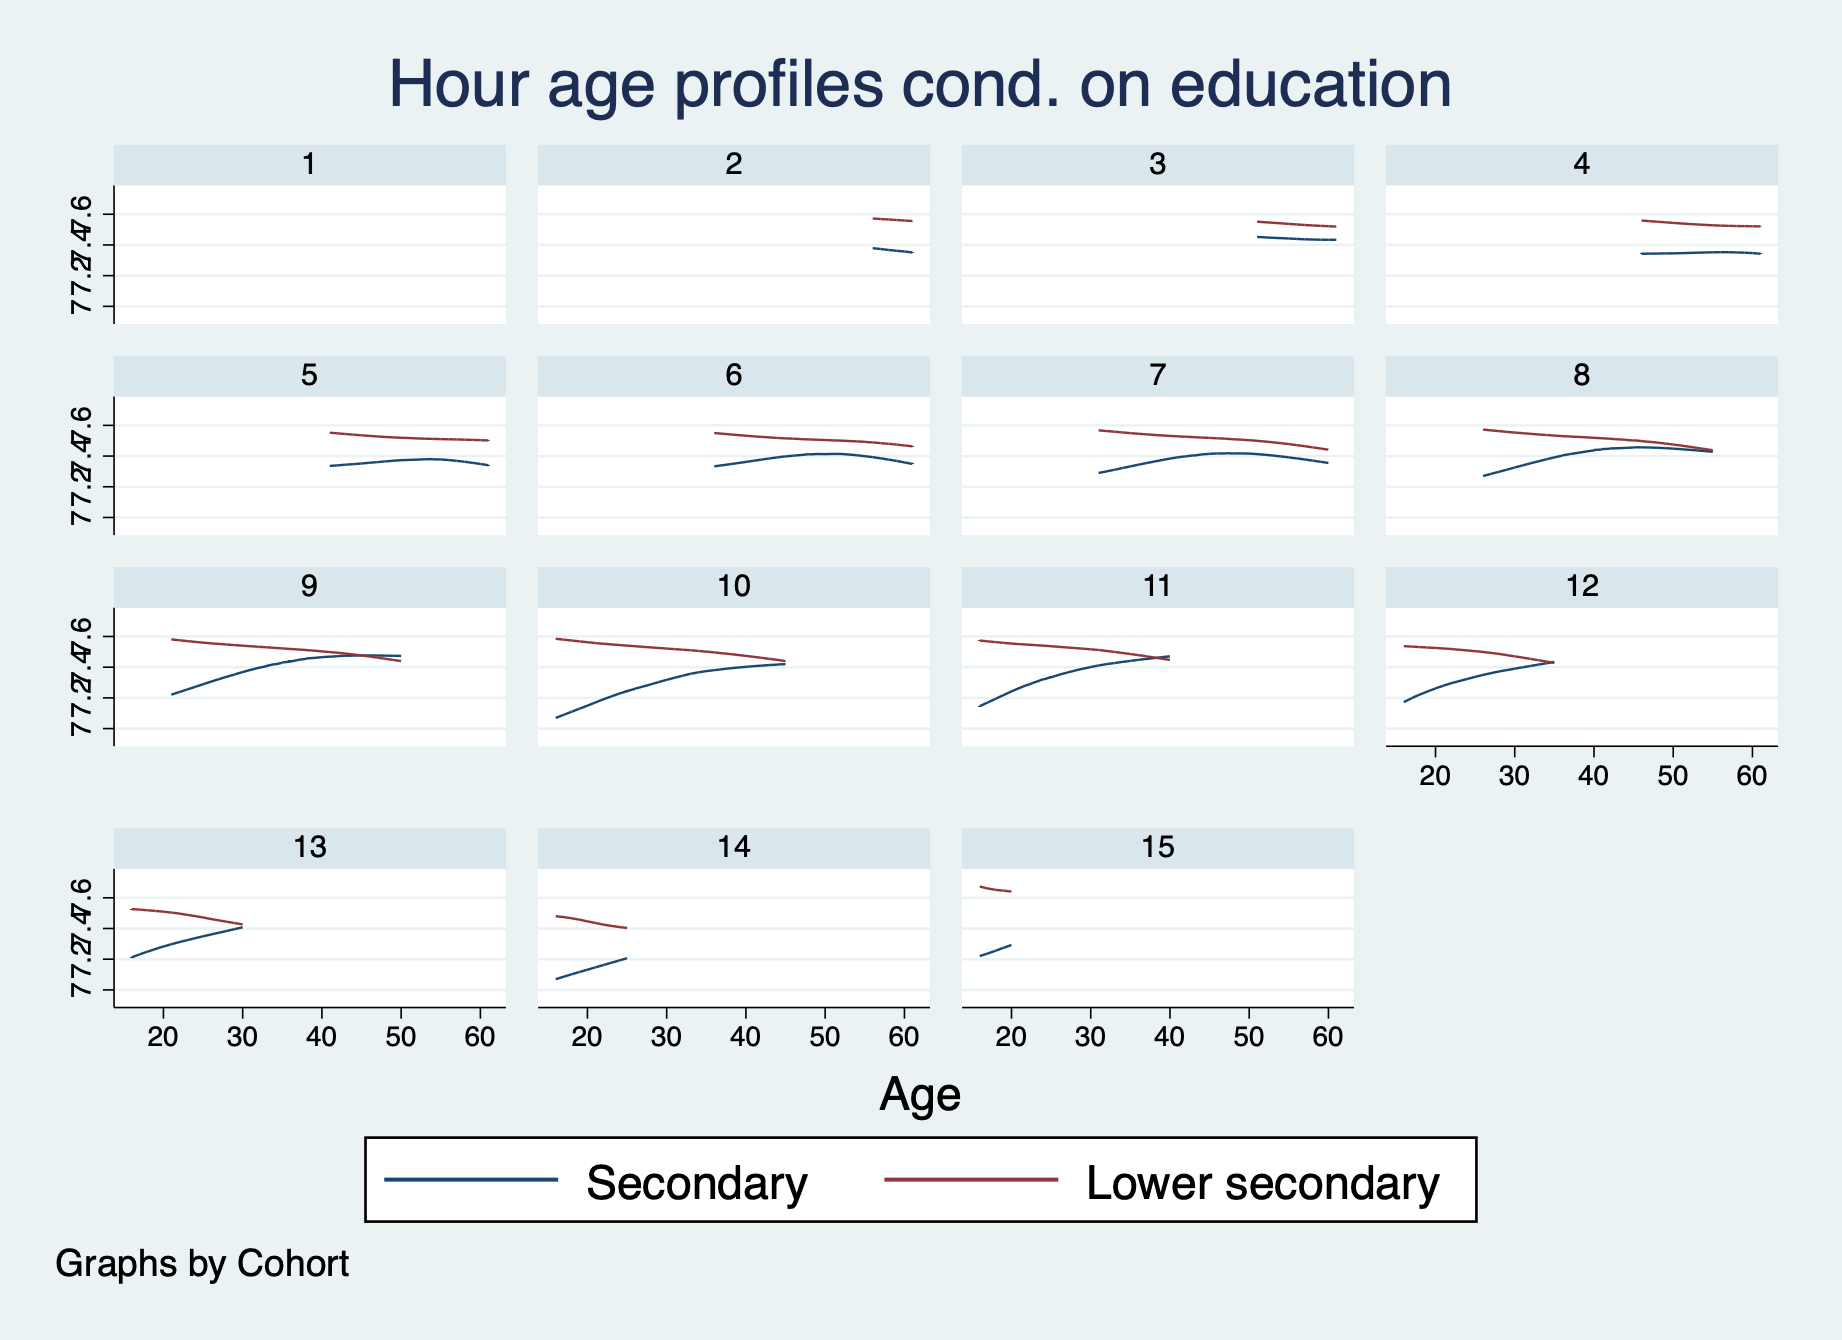
\includegraphics[scale=0.4]{graph4.png}
    \caption{\label{fig:hours}Hours-age profile}
\end{figure}
\begin{figure}[!h]
    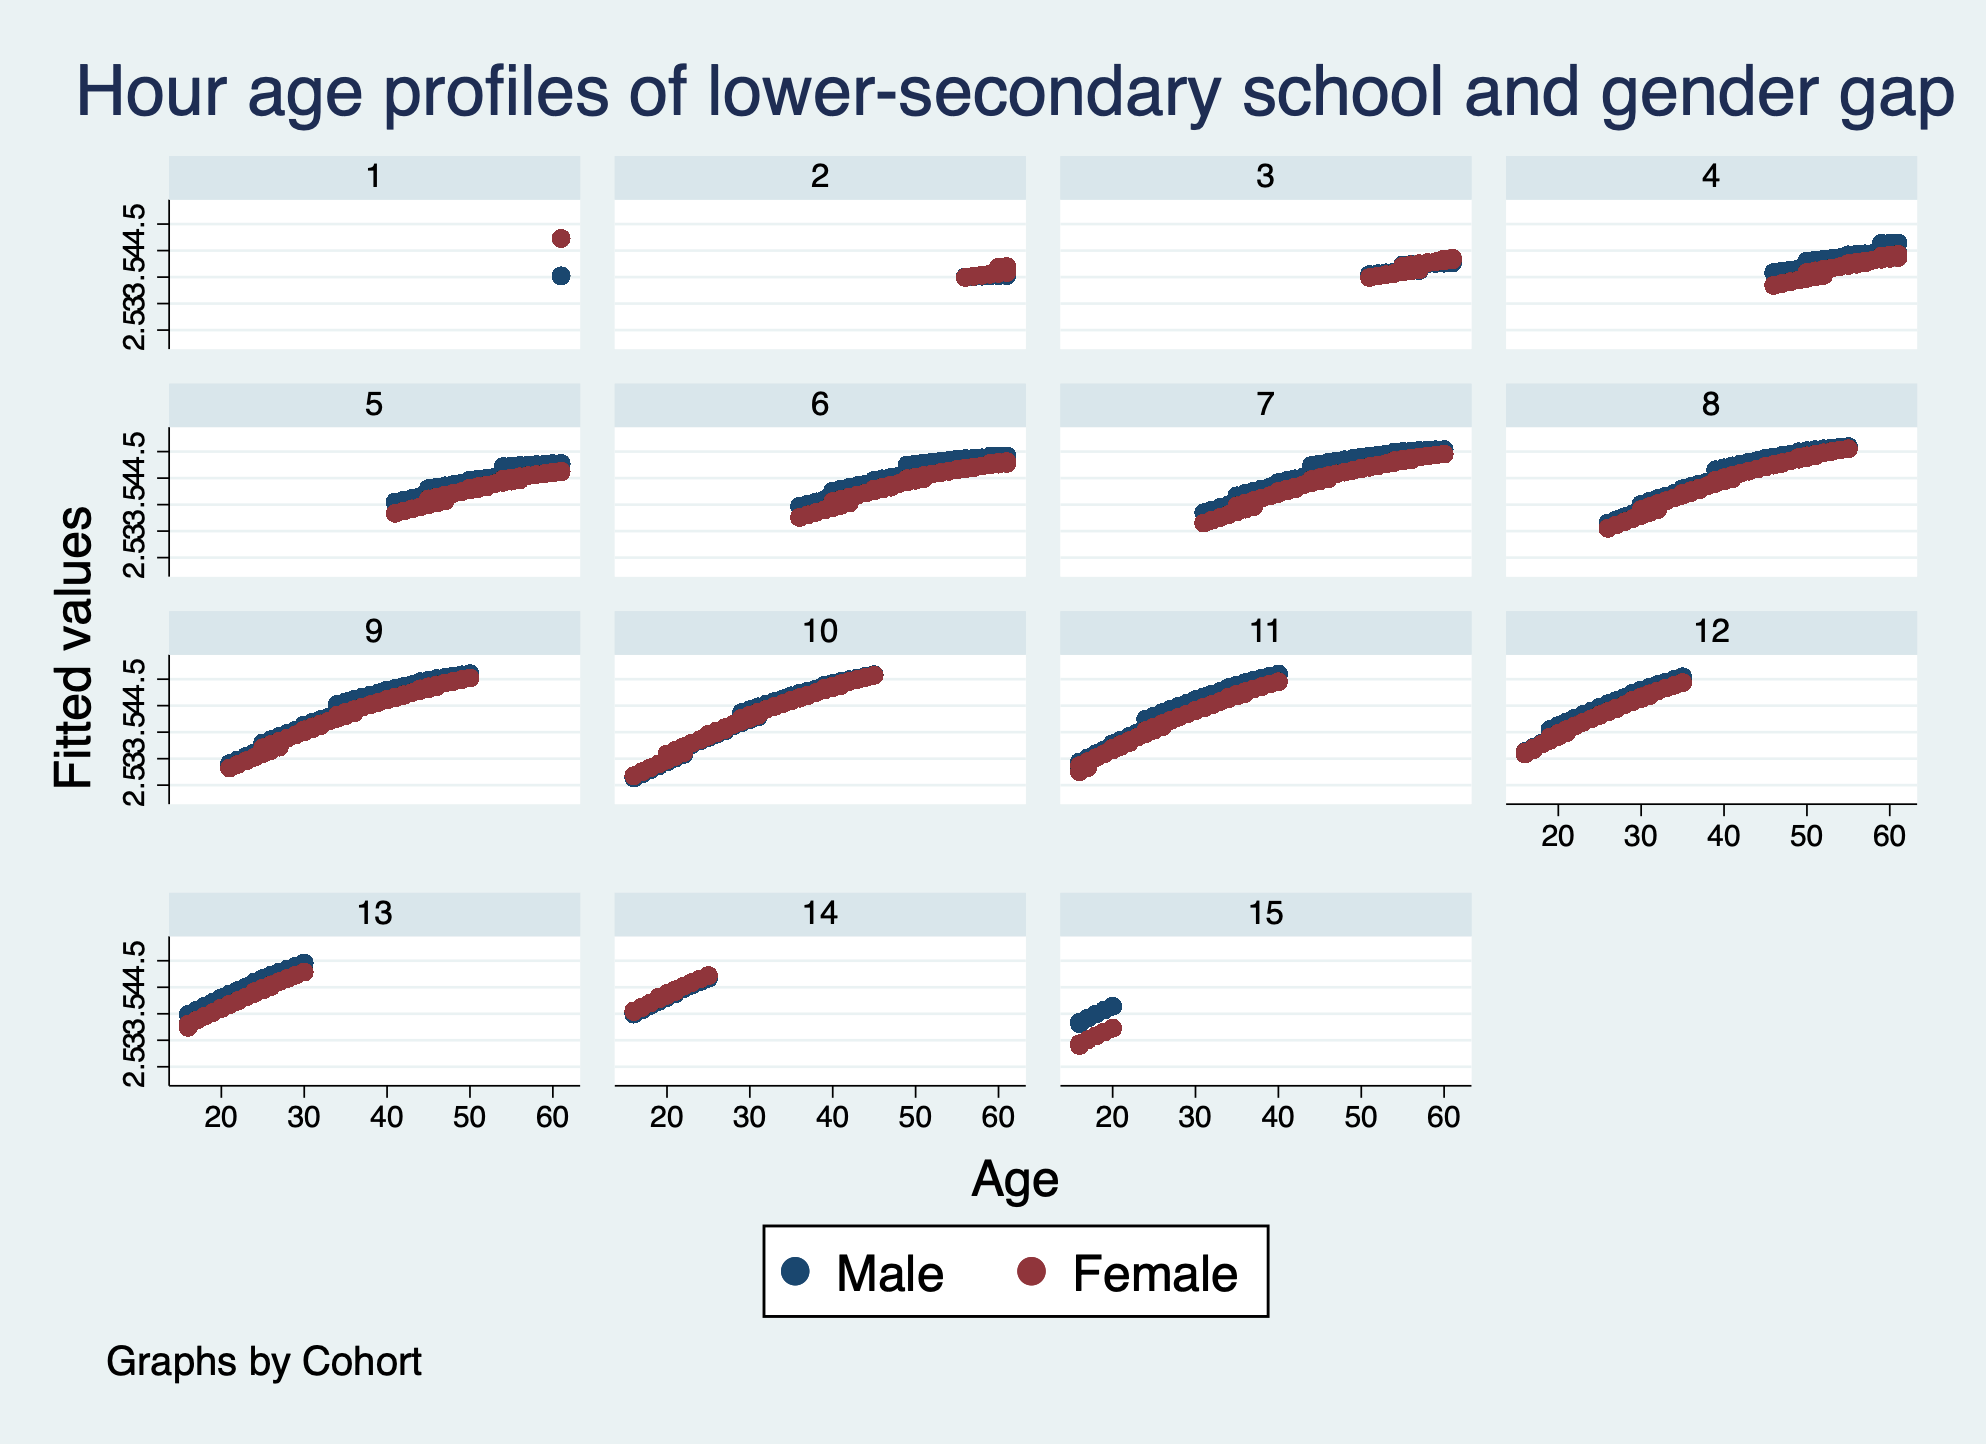
\includegraphics[scale=0.35]{graph5.png}
    \caption{\label{fig:h_l_cohorts}Hours-age profile and gender gap}
\end{figure}
\begin{figure}[!h]
    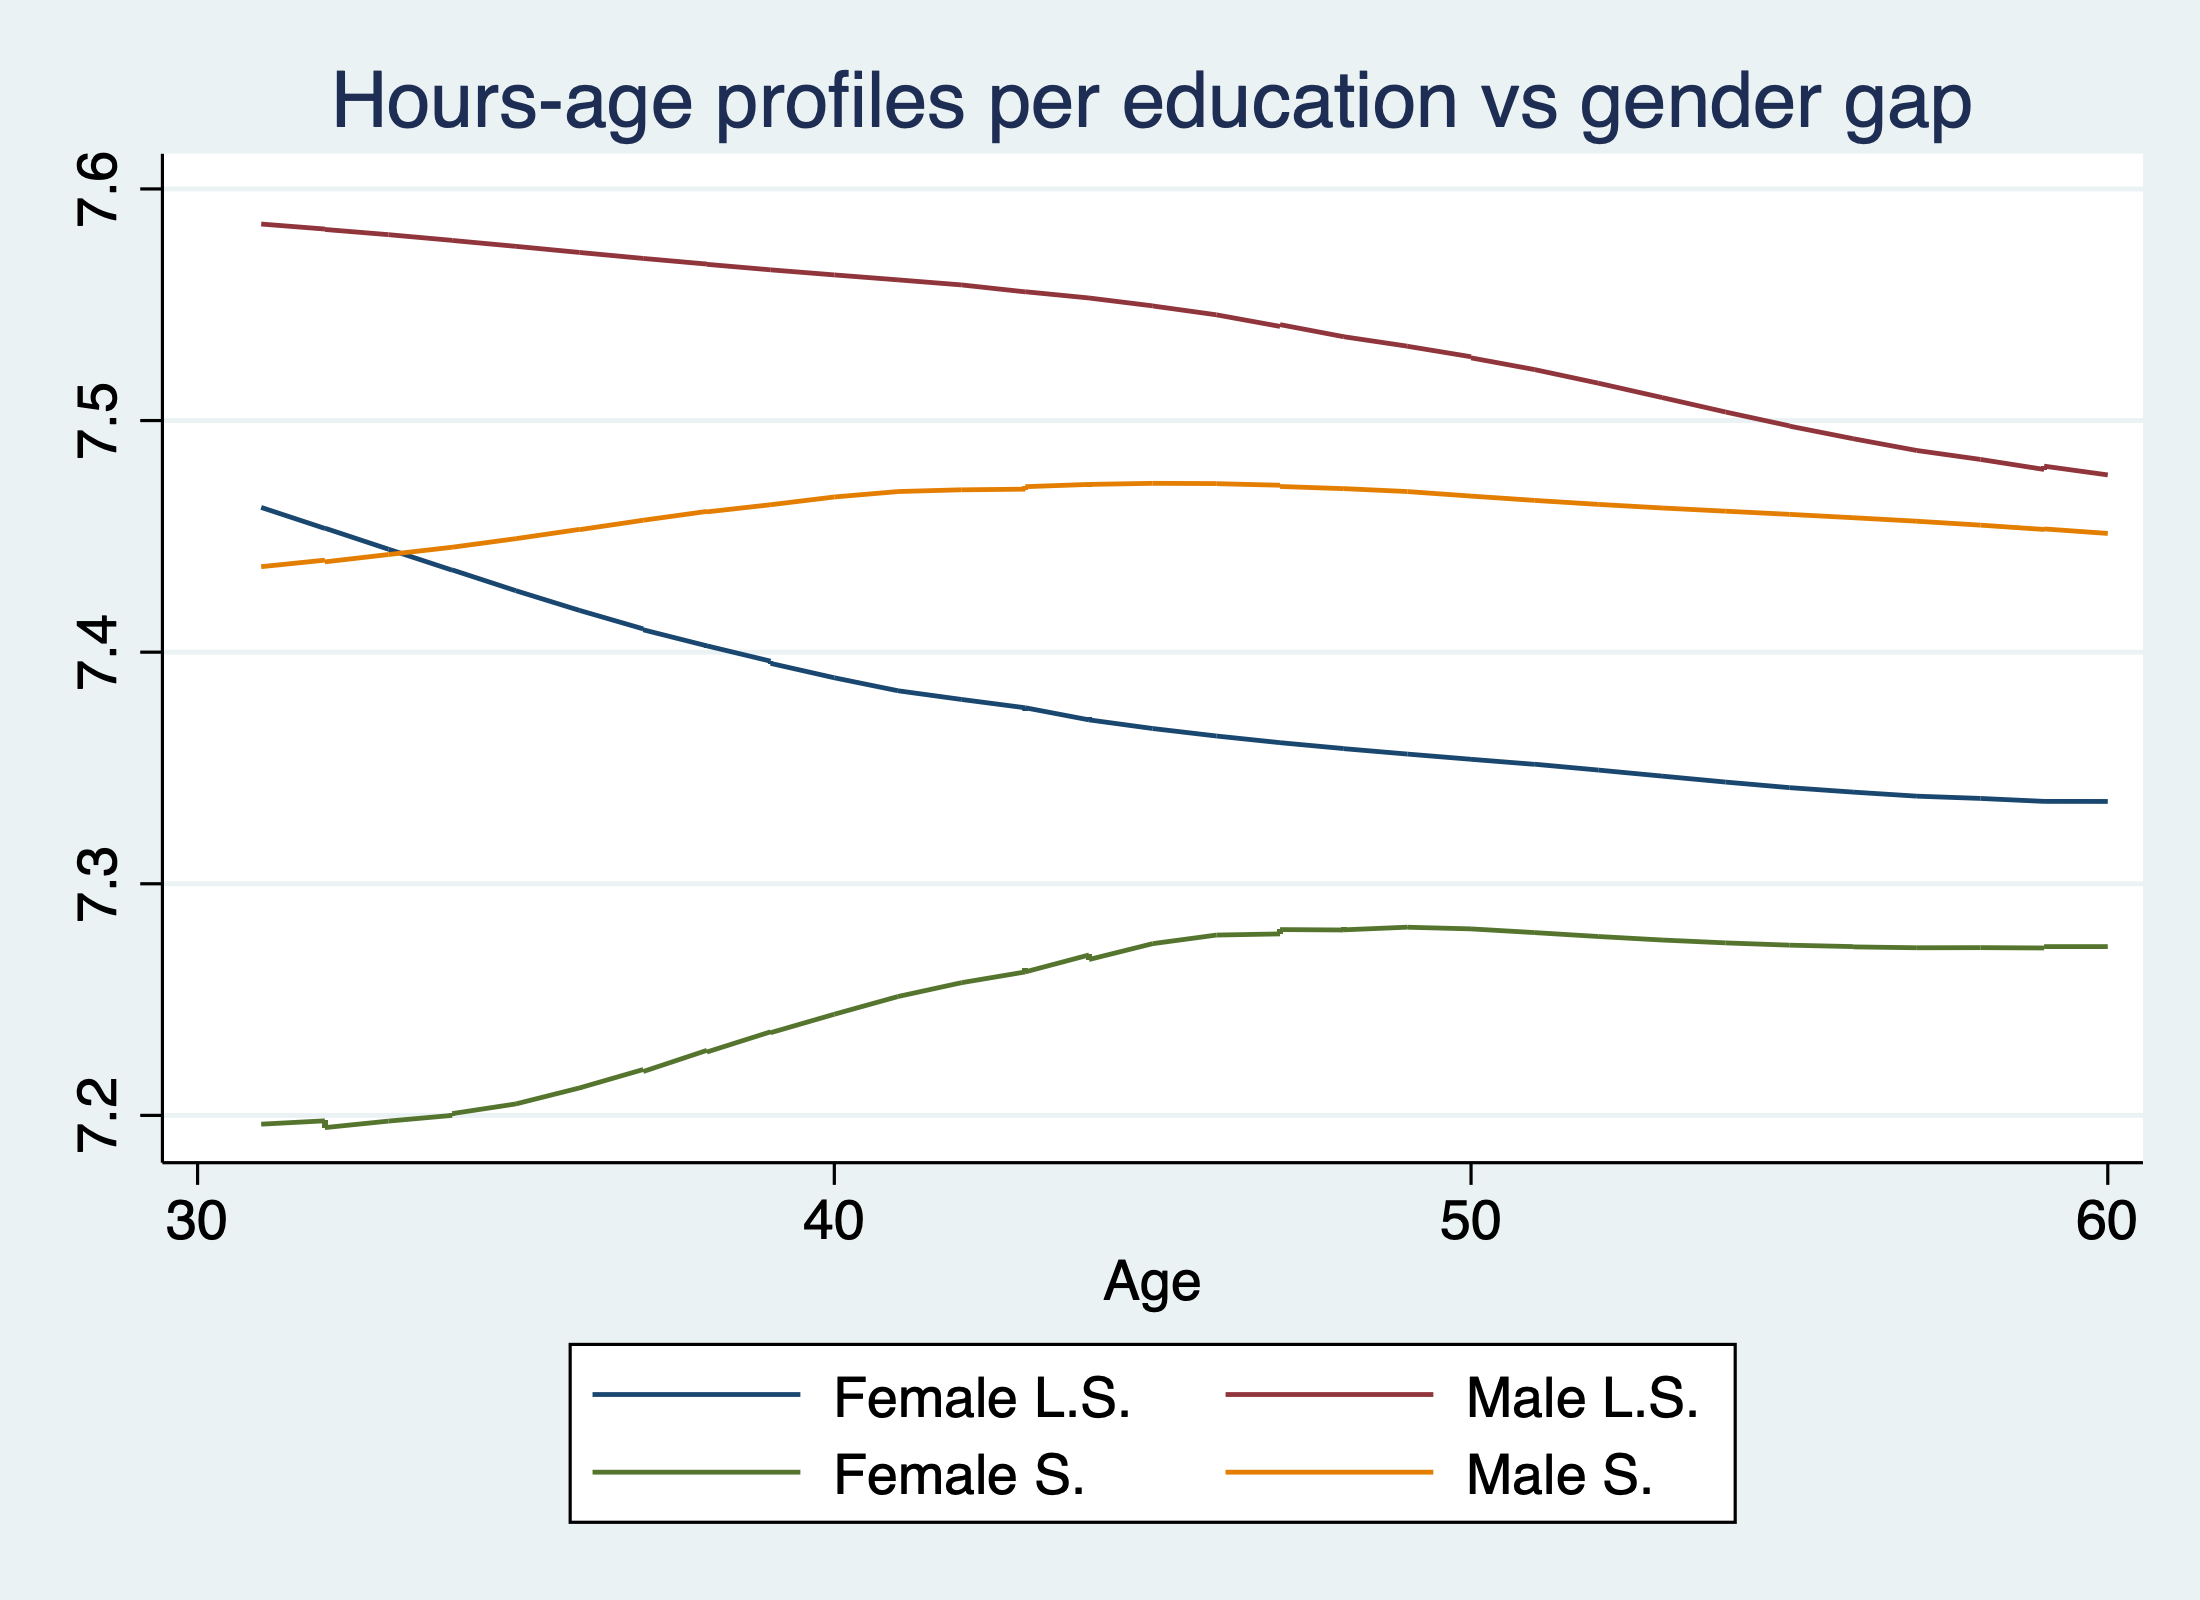
\includegraphics[scale=0.35]{graph5_1.png}
    \caption{\label{fig:h_l_coh8}Hours-age profile and gender gap in the cohort 8}
\end{figure}
\end{center}




 

\end{document}


